\documentclass[10pt, letterpaper]{article}
\usepackage[utf8]{inputenc}
\usepackage{amsmath}
\usepackage{amssymb}
\usepackage{bbm}
\usepackage{booktabs}
\usepackage{caption}
\usepackage{color}
\usepackage[shortlabels]{enumitem}
\usepackage{fancyhdr}
\usepackage{hyperref}
\usepackage{geometry}
\geometry{a4paper,scale=0.8}
\usepackage{graphicx}
\graphicspath{ {./img/}}
\usepackage{listings}
\usepackage{mathtools}
\usepackage{mathrsfs}
\usepackage{setspace}
\usepackage{subfigure}
\renewcommand{\baselinestretch}{1.3}

% set-up header & footer
\pagestyle{empty}
\fancyhf{}
\cfoot{\thepage}
\lhead{%
\textbf{University of California, Berkeley} \\
Department of Civil \& Environ. Eng.
}
\rhead{\textbf{CS 285 Deep Reinforcement Learning}\\\date{\today}}

\title{%
    \textbf{Homework 5}
}
\author{Juanwu Lu (3037432593)\\ \small(M.Sc. Civil Engineering, UC Berkeley)}
\date{}

% set-up code listing
\definecolor{dkgreen}{rgb}{0,0.6,0}
\definecolor{gray}{rgb}{0.5,0.5,0.5}
\definecolor{manuve}{rgb}{0.58,0,0.82}

\lstset{frame=tb,
    language=Python,
    aboveskip=3mm,
    belowskip=3mm,
    showstringspaces=false,
    columns=flexible,
    basicstyle={\small\ttfamily},
    numbers=none,
    numberstyle=\tiny\color{gray},
    keywordstyle=\color{blue},
    commentstyle=\color{dkgreen},
    stringstyle=\color{manuve},
    breaklines=true,
    breakatwhitespace=true,
    tabsize=3
}

\begin{document}
\maketitle
\captionsetup[figure]{labelfont={bf},labelformat={default},labelsep=period,name={Figure}}
\captionsetup[table]{labelfont={bf},labelformat={default},labelsep=period,name={TABLE}}
\thispagestyle{fancy}
\pagestyle{plain}

% Problem 1
\section*{Problem 1 "Unsupervised" RND and exploration performance}
\subsection*{Part 1 Results}

\begin{figure}[h!]
    \centering
    \subfigure[]{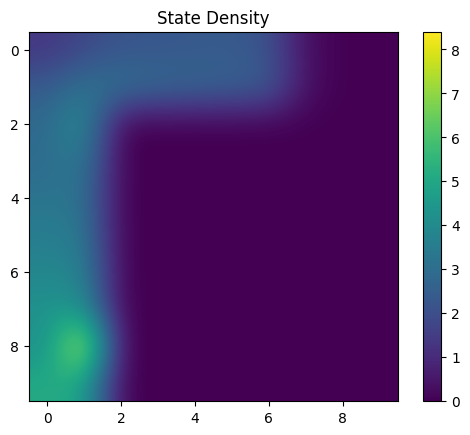
\includegraphics[width=0.35\textwidth]{q1_easy_random.png}}
    \subfigure[]{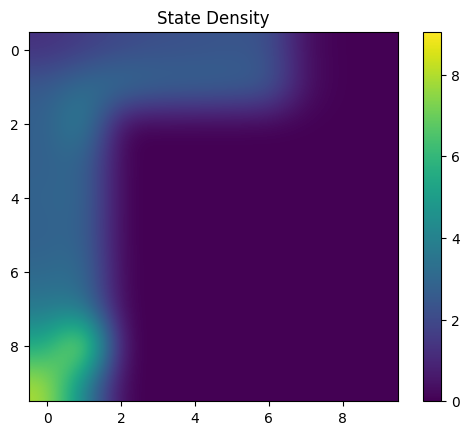
\includegraphics[width=0.35\textwidth]{q1_easy_rnd.png}}
    \caption{Results from PointmassEasy Environment: (a) Random exploration with epsilon-greedy; (b) Exploration with RND. State density of from the two algorithms are similar but RND unexpectedly has a denser density around the lower left corner (origin).}
    \label{fig:1}
\end{figure}

\begin{figure}[h!]
    \centering
    \subfigure[]{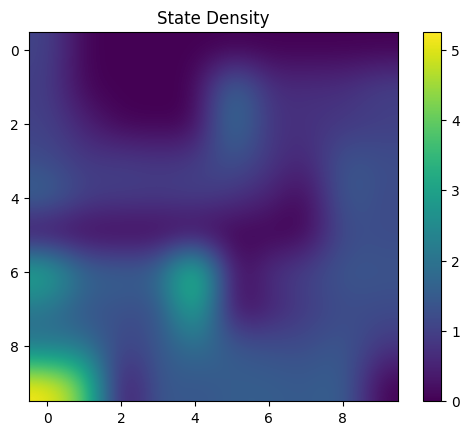
\includegraphics[width=0.35\textwidth]{q1_medium_random.png}}
    \subfigure[]{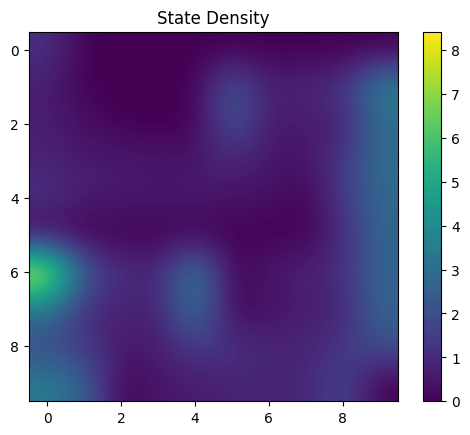
\includegraphics[width=0.35\textwidth]{q1_medium_rnd.png}}
    \caption{Results from PointmassMedium Environment: (a) Random exploration with epsilon-greedy; (b) Exploration with RND. State density of from the two algorithms are similar but RND has a more uniformly distributed density than the random exploration one.}
    \label{fig:2}
\end{figure}

\begin{figure}[h!]
    \centering
    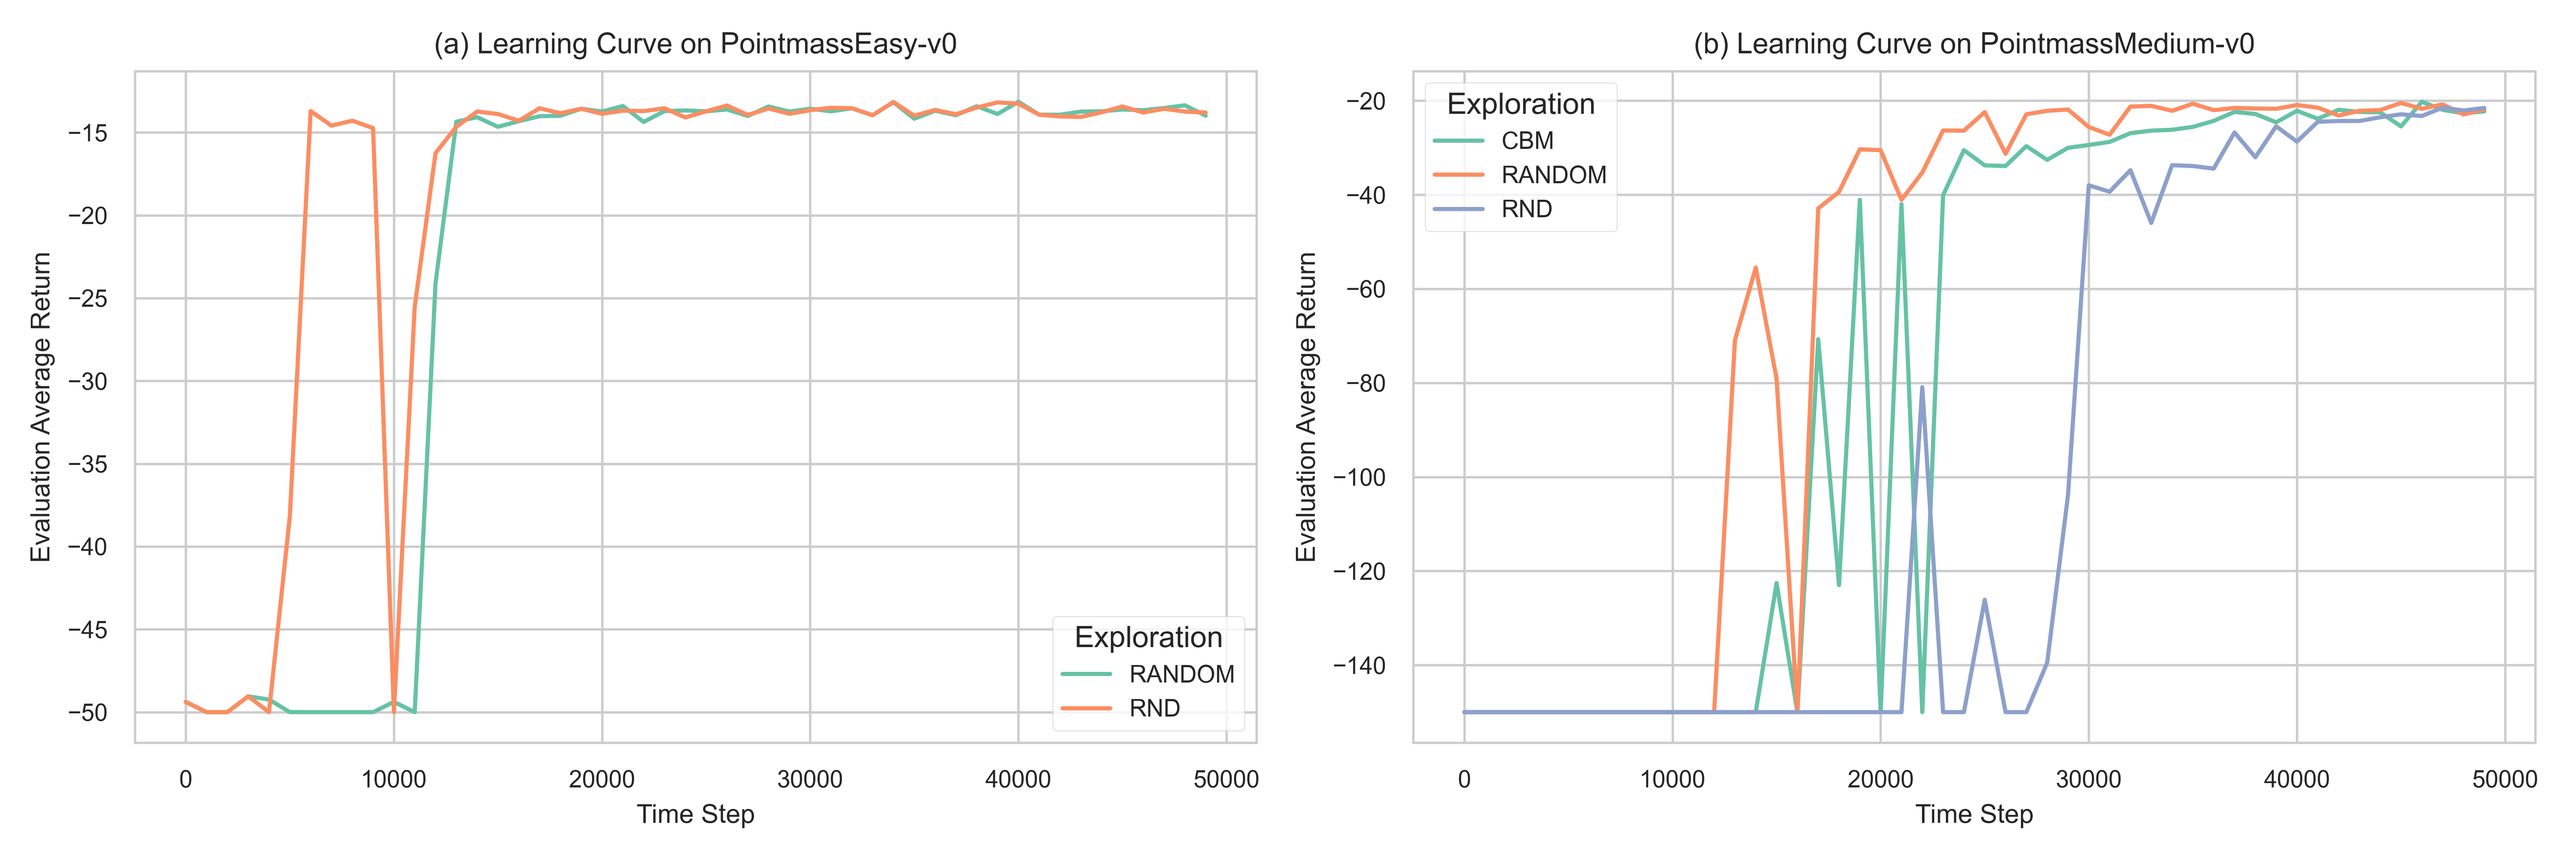
\includegraphics[width=\textwidth]{q1_learning_curve.png}
    \caption{Learning curve from the two environments. RND reaches higher score faster than epsilon-greedy on the PointmassEasy environment, while slower on the PointmassMedium environment.}
    \label{fig:3}
\end{figure}

\subsection*{Part 2 Results}

Since the state space is a grid world. I implemented the UCB-like count-based exploration (CBM), where 
\begin{equation}
    r_{\text{explore}}(s) = N(s)^{-\frac{1}{2}}
\end{equation}
As shown in \hyperref[fig:3]{Figure 3}, DQN with CBM learns faster than the RND, but slower than the epsilon-greedy. From the figures below, I think this is partly because it's exploring more states than the epsilon-greedy algorithm.

\begin{figure}[h!]
    \centering
    \subfigure[]{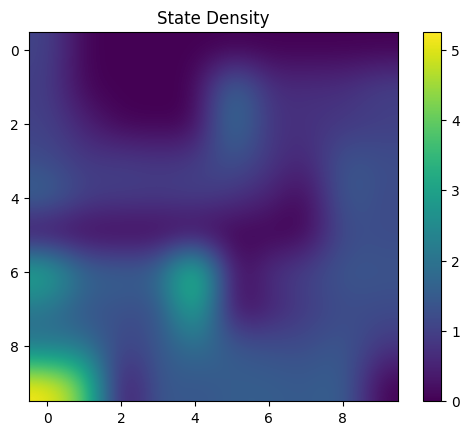
\includegraphics[width=0.3\textwidth]{q1_medium_random.png}}
    \subfigure[]{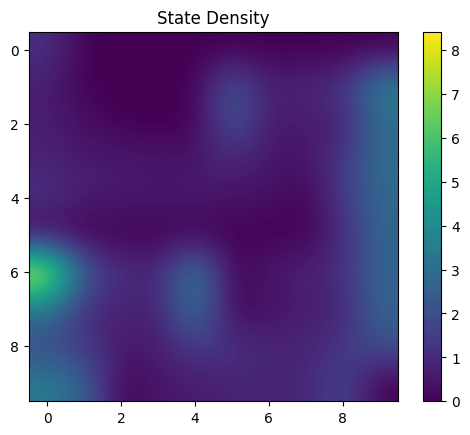
\includegraphics[width=0.3\textwidth]{q1_medium_rnd.png}}
    \subfigure[]{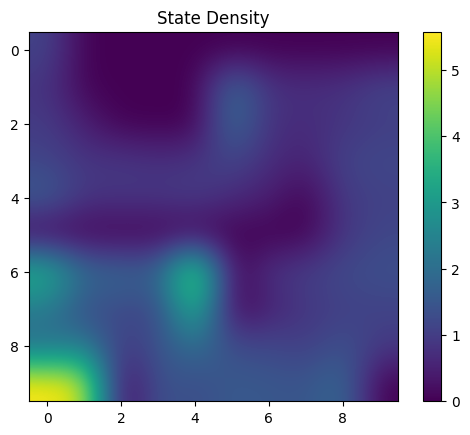
\includegraphics[width=0.3\textwidth]{q1_medium_alg.png}}
    \caption{Results from PointmassMedium Environment: (a) Random exploration with epsilon-greedy; (b) Exploration with RND; (c) Exploration with count-based Model. State density from epsilon-greed and count-based exploration strategies are quite similar, while the one from RND-based exploration is more uniformly distributed.}
    \label{fig:4}
\end{figure}


\pagebreak
\section*{Problem 2 Offline learning on exploration data}
\subsection*{Part 1 Compare CQL to DQN on the \texttt{PointmassMedium} environment}

\begin{figure}[h!]
    \centering 
    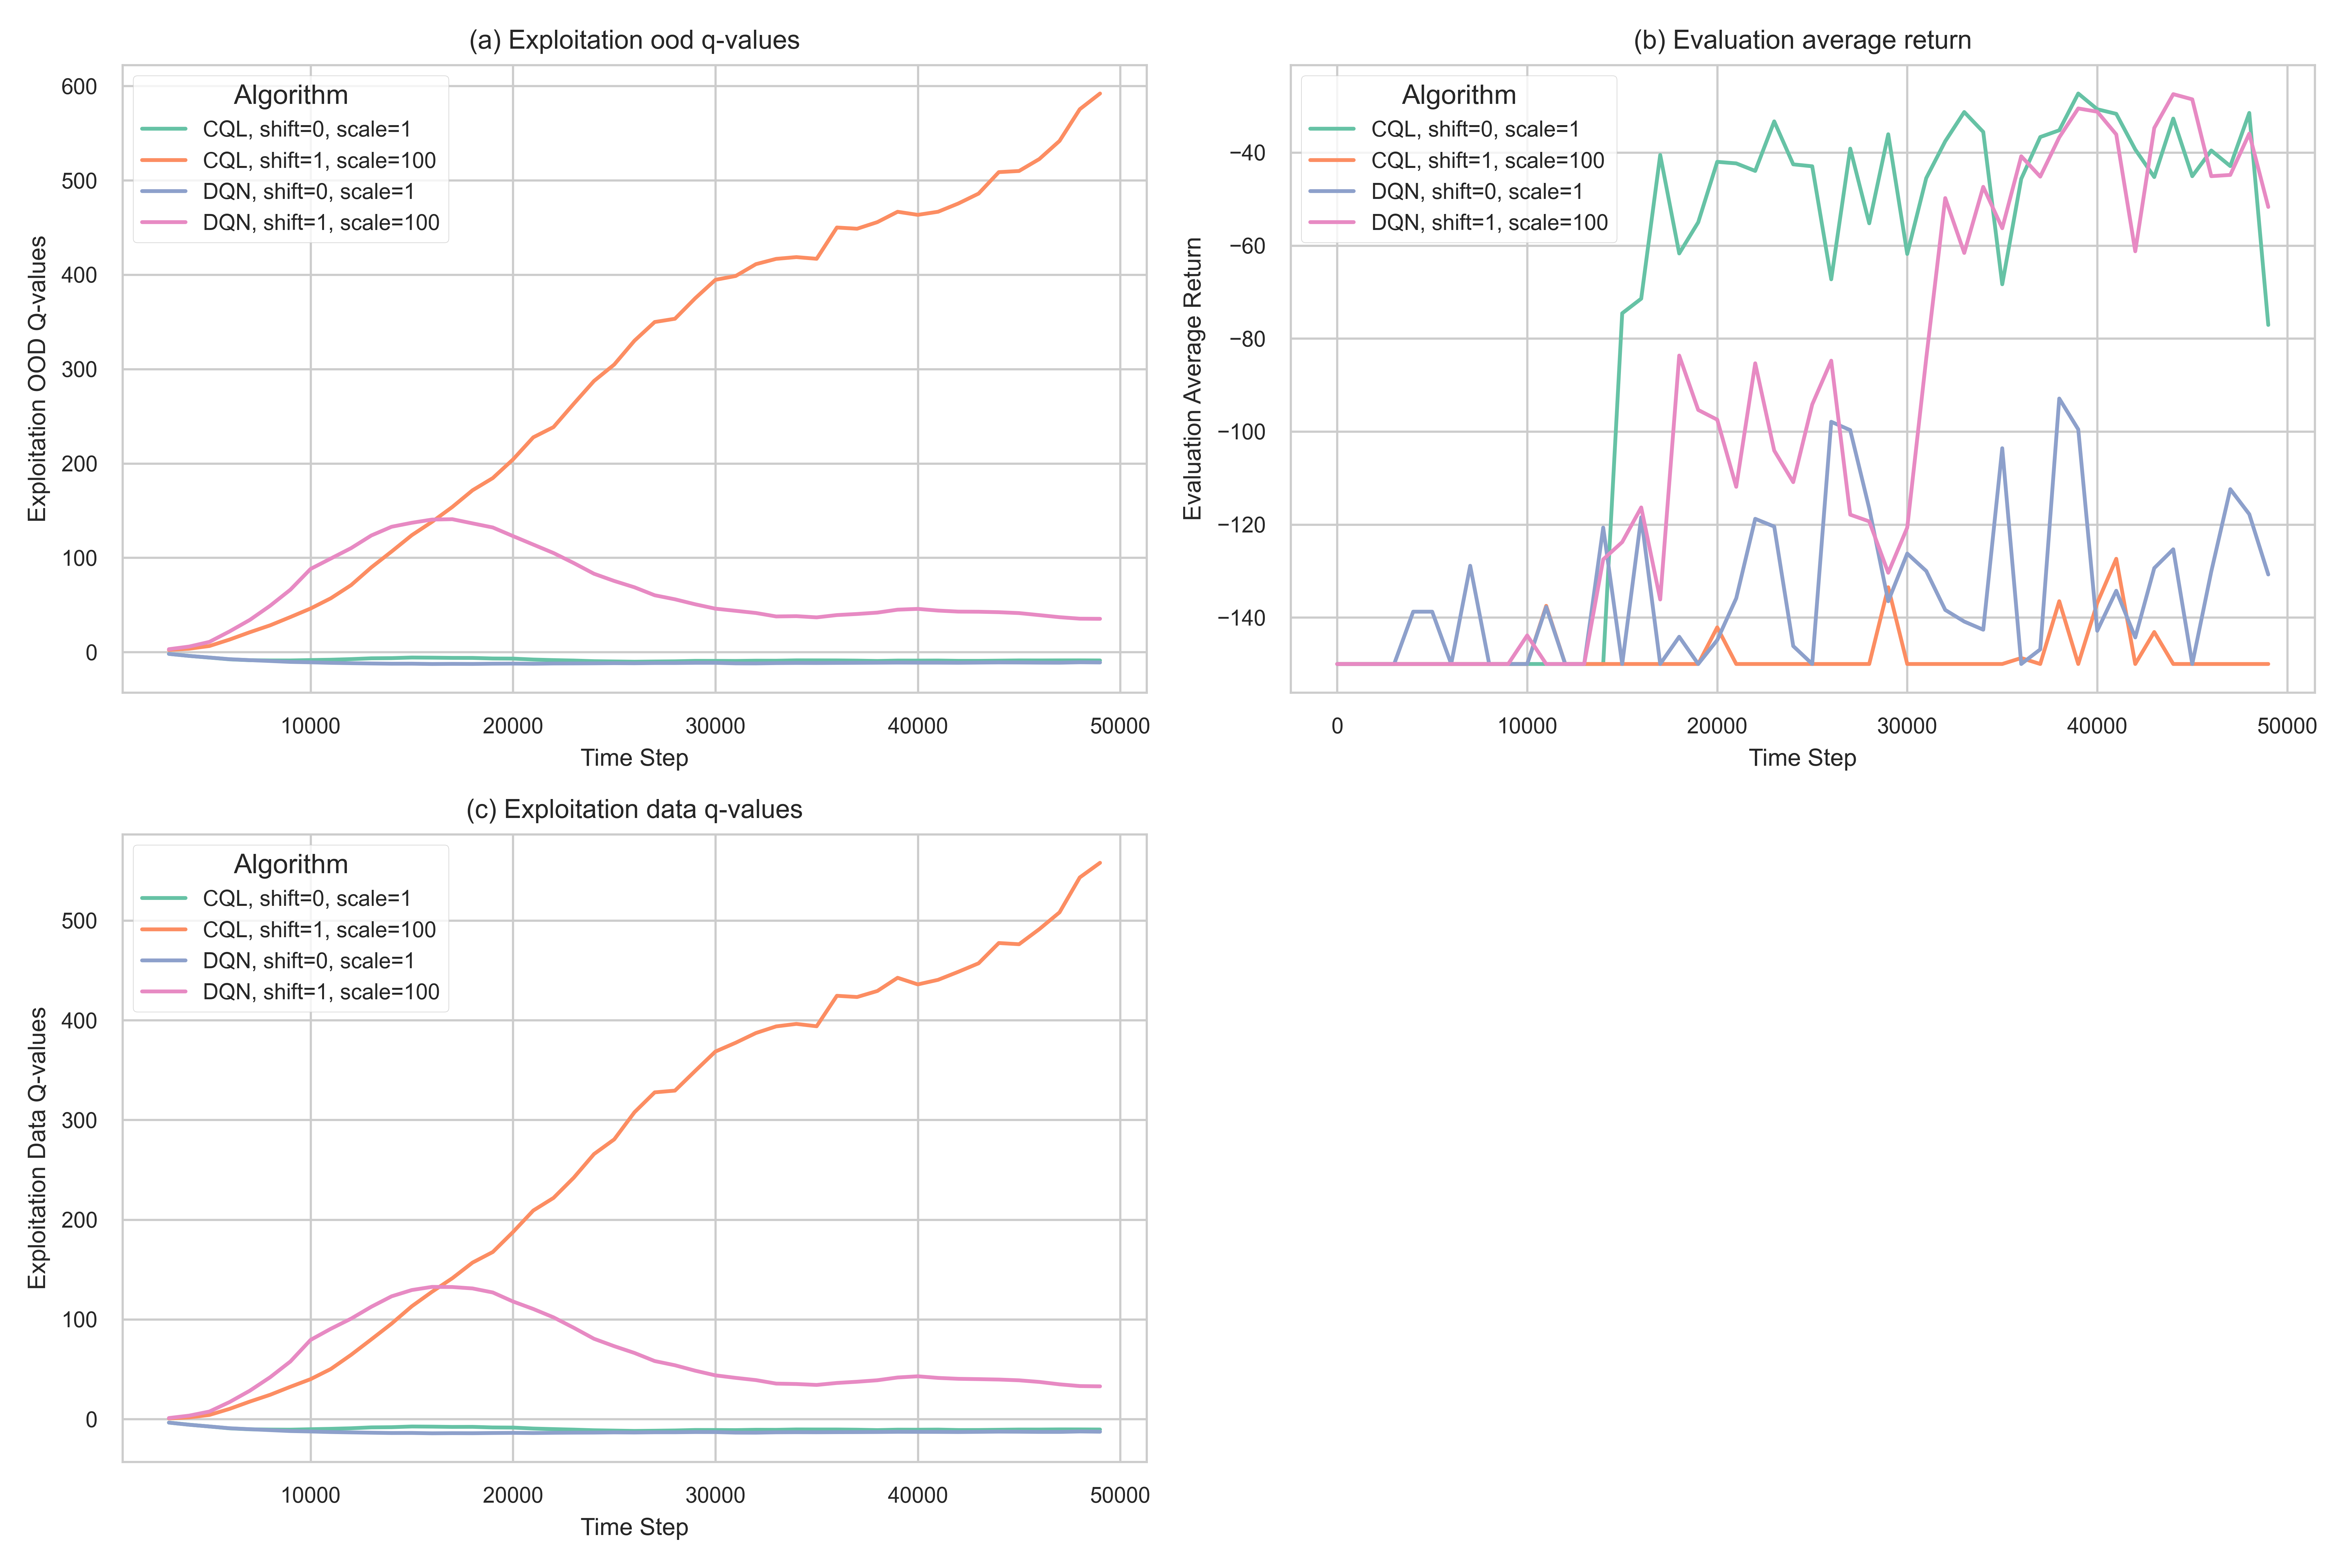
\includegraphics[width=\textwidth]{q2_1.png}
    \caption{(a) OOD Q-value estimation; (b) Evaluation Average Returns; and (c) Buffer Q-value estimation on DQN- and CQL-based algorithm with/without reward scale and shifts. My experiment results shows that CQL works better with the original reward with only penalties of -1, while DQN works better with scale and shifted rewards. With the original reward settings, CQL helps to prevent overestimation of OOD Q values, while it fails with scaled and shifted rewards. My explanation to this is that shifting and scaling with 1 and 100 causes rewards to be more sparse (i.e., only getting 100 when success while getting 0 at other places). This mitigate overestimation of OOD Q values for DQN, which helps it perform better.}
\end{figure}



\subsection*{Part 2 Ablation study on amount of exploration data}

\begin{table}[h!]
    \centering
    \caption{Final average evaluation return of DQN- and CQL-based exploration with different exploration steps. Surprisingly, my experiment results indicate that increasing the number of unsupervised exploration steps in return deteriorate the learning performance. And DQN-based algorithm worsen much more significantly than the CQL-based one. My explanation for this is that unsupervised exploration can actually generate a series of out-of-distribution data. Given sparse rewards, it actually makes it more difficult to learn from the exploration data. And DQN can overestimate the Q values of some OOD data, which cause a even worse performance.}
    \begin{tabular}{lcc}
        \hline
        \multicolumn{1}{c}{\textbf{Number of Exploration Steps}} & \textbf{DQN} & \textbf{CQL} \\ \hline
        5000                                                     & -36.75       & -30.73       \\
        15000                                                    & -127.4       & -75.33       \\ \hline
    \end{tabular}
\end{table}

\subsection*{Part 3 Ablation study on the regularizer weight $\alpha$}

\begin{figure}[h!]
    \centering
    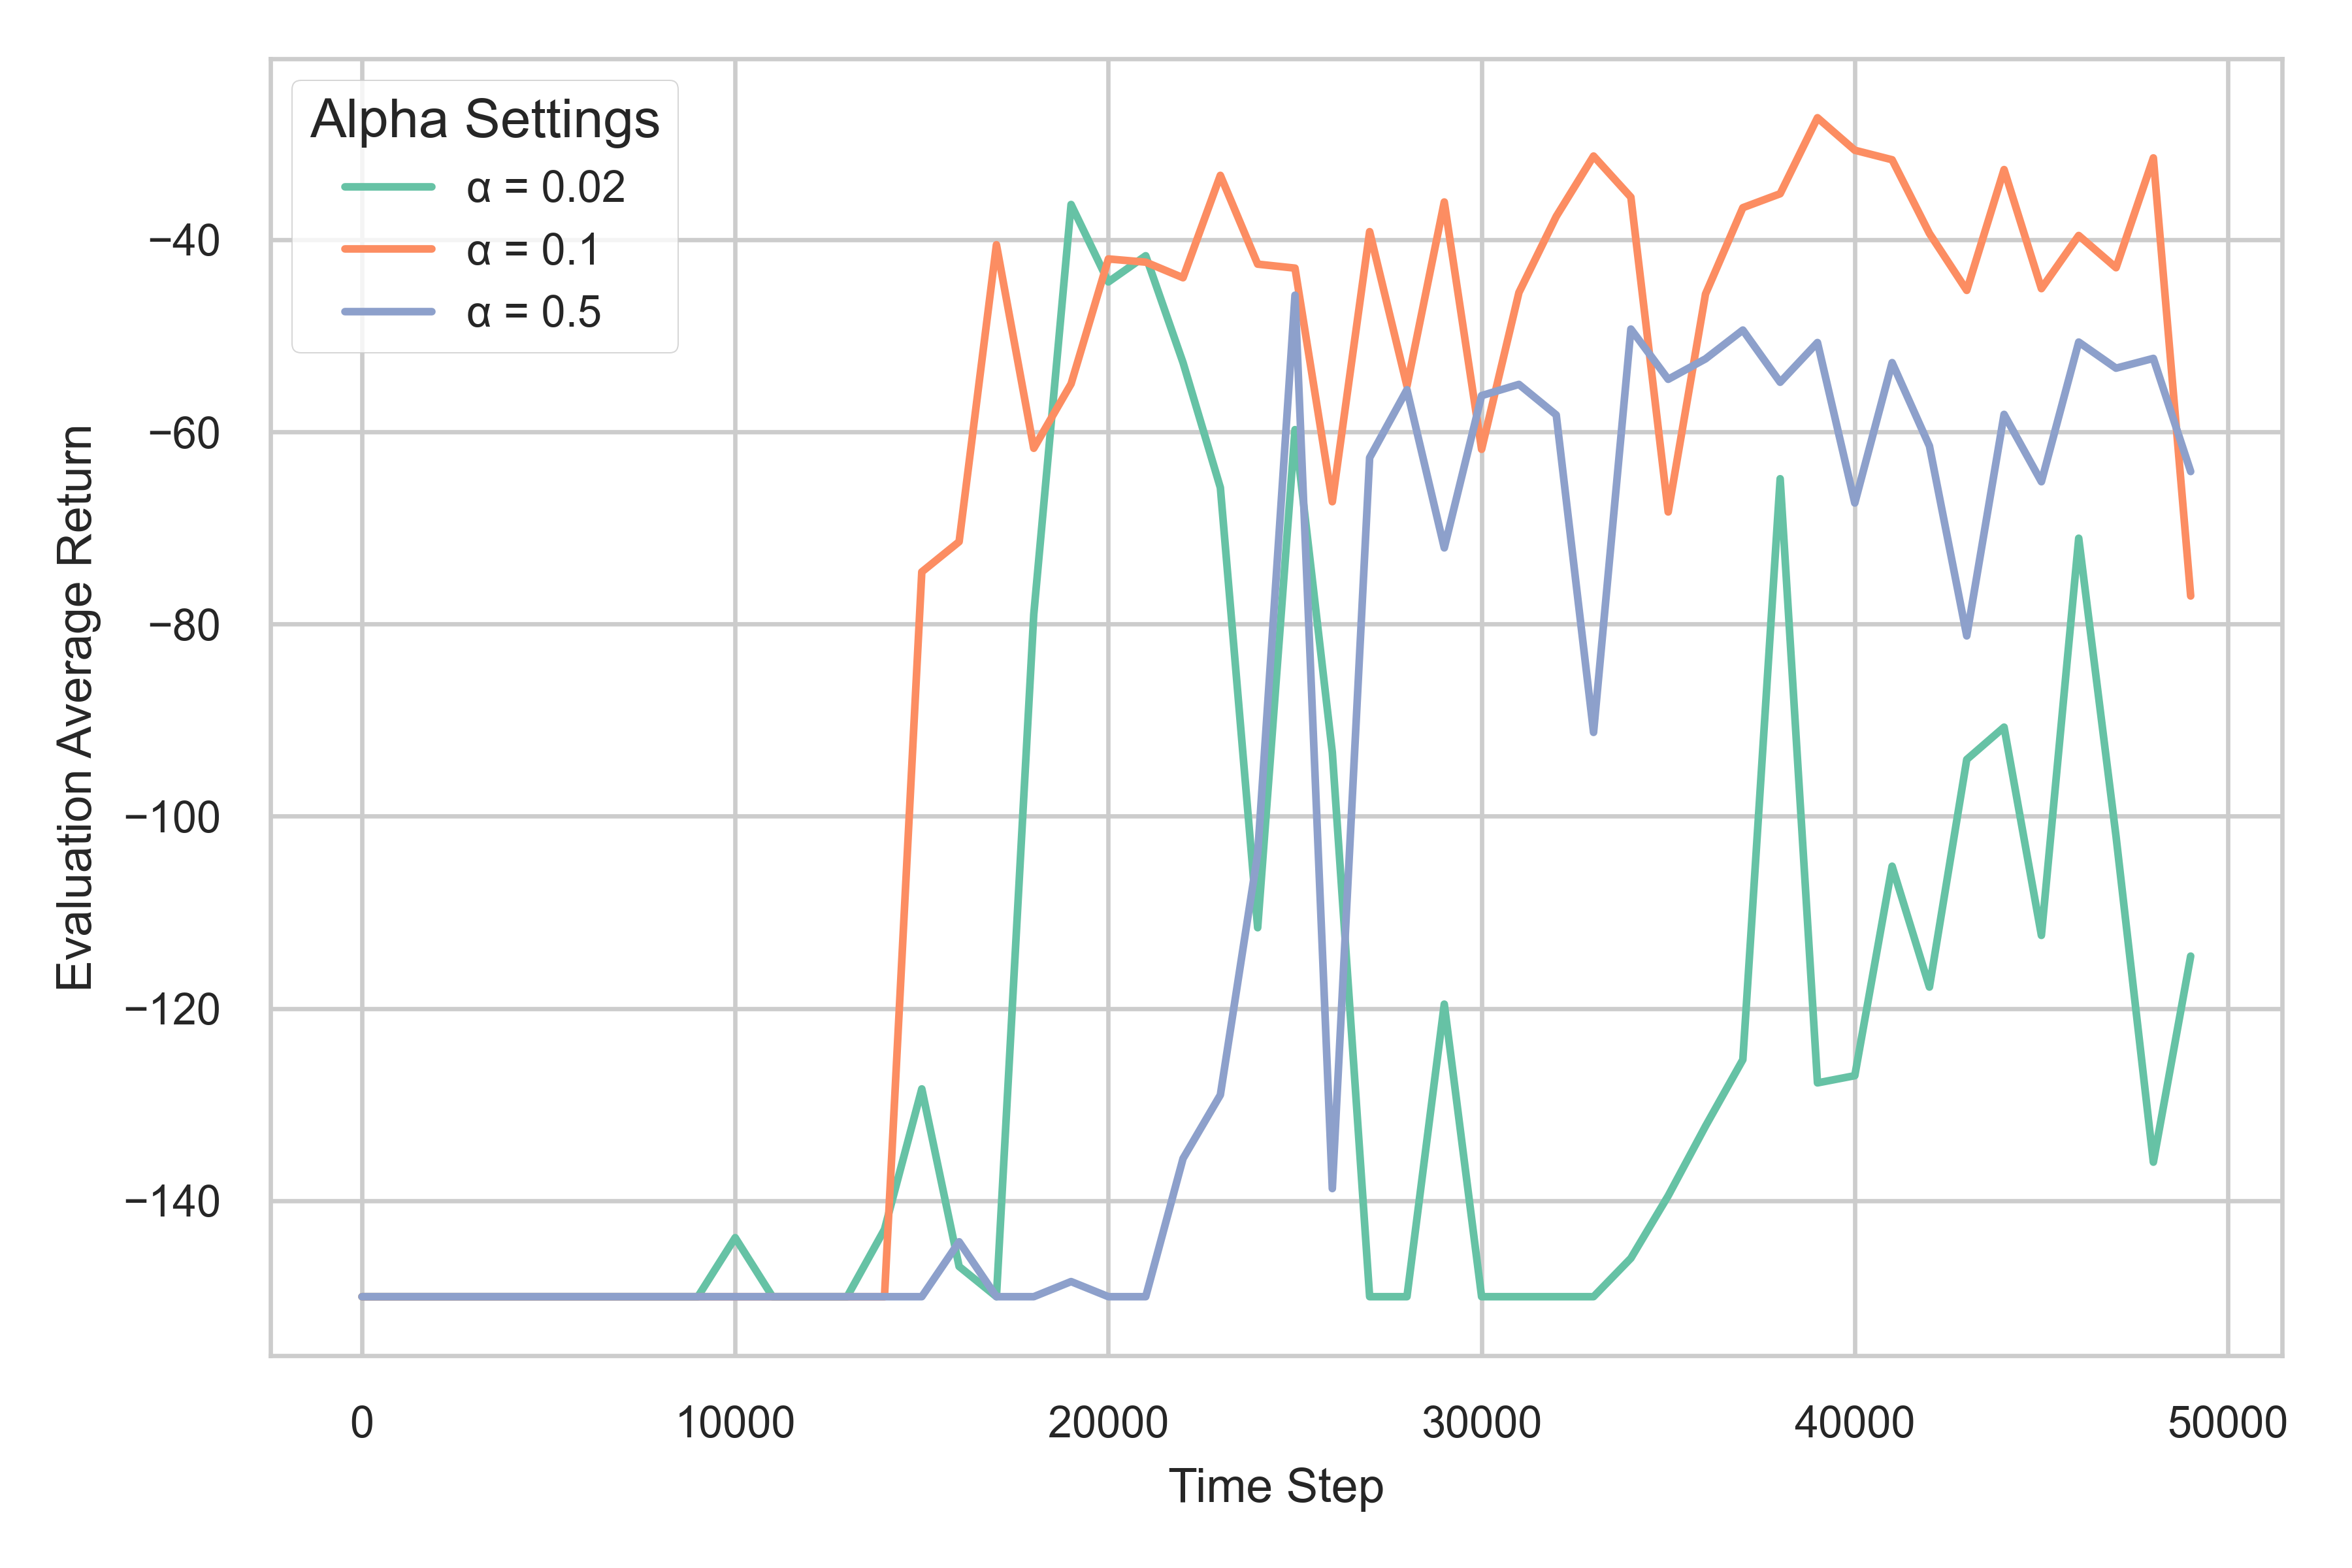
\includegraphics[width=\textwidth]{q2_3.png}
    \caption{Learning curve of CQL-based algorithm on \texttt{PointmassMedium} with different $\alpha$ settings. From its formulation, higher value of $\alpha$ promotes stronger constraints on overestimation of the OOD q-value, which results in a more conservative. Therefore, the figure shows that with smaller $\alpha$ value, the algorithm tends to reach higher score earlier, but finds it hard to maintain the achievement since it tends to overestimate some OOD states. On the contrary, a higher $\alpha$ value would cause a longer time to train, but the learning curve is more stable at the end.}
\end{figure}

\pagebreak
\section*{Problem 3 "Supervised" exploration with mixed reward bonuses}

\begin{figure}[h!]
    \centering
    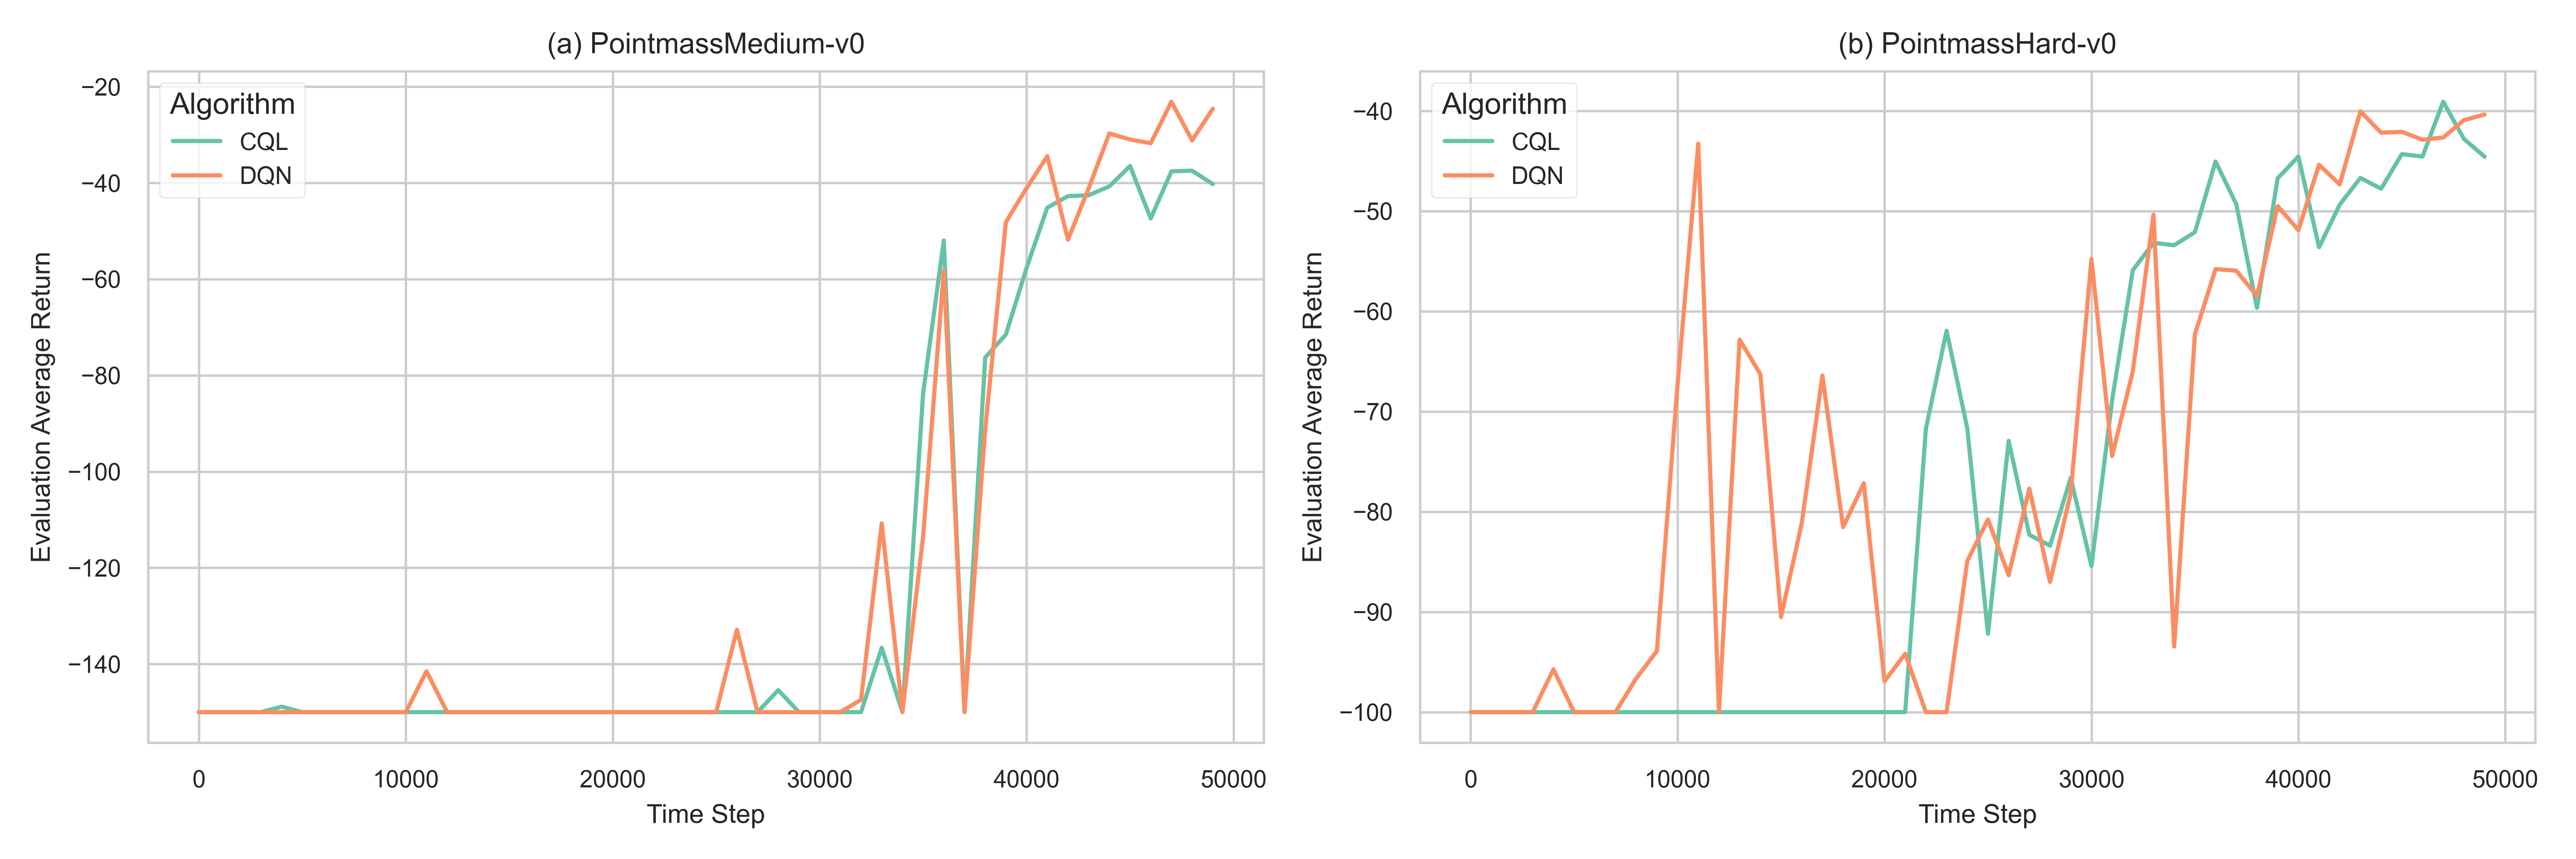
\includegraphics[width=\textwidth]{q3.png}
    \caption{Learning curve of DQN- and CQL-based exploitation algorithms on (a) \texttt{PointmassMedium} and (b) \texttt{PointmassHard} environments.  Compared to the results in Part 1, supervised exploration helps stablize the learning curve and is more effective regarding the convergence. The reason I can think of is that supervised exploration has a changing weighting of exploration vs. exploitation, which helps the algorithms to adjust its strategy across different learning period to explore more effectively.}
\end{figure}

\pagebreak
\section*{Problem 4 Offline Learning with AWAC}

\begin{figure}[h!]
    \centering
    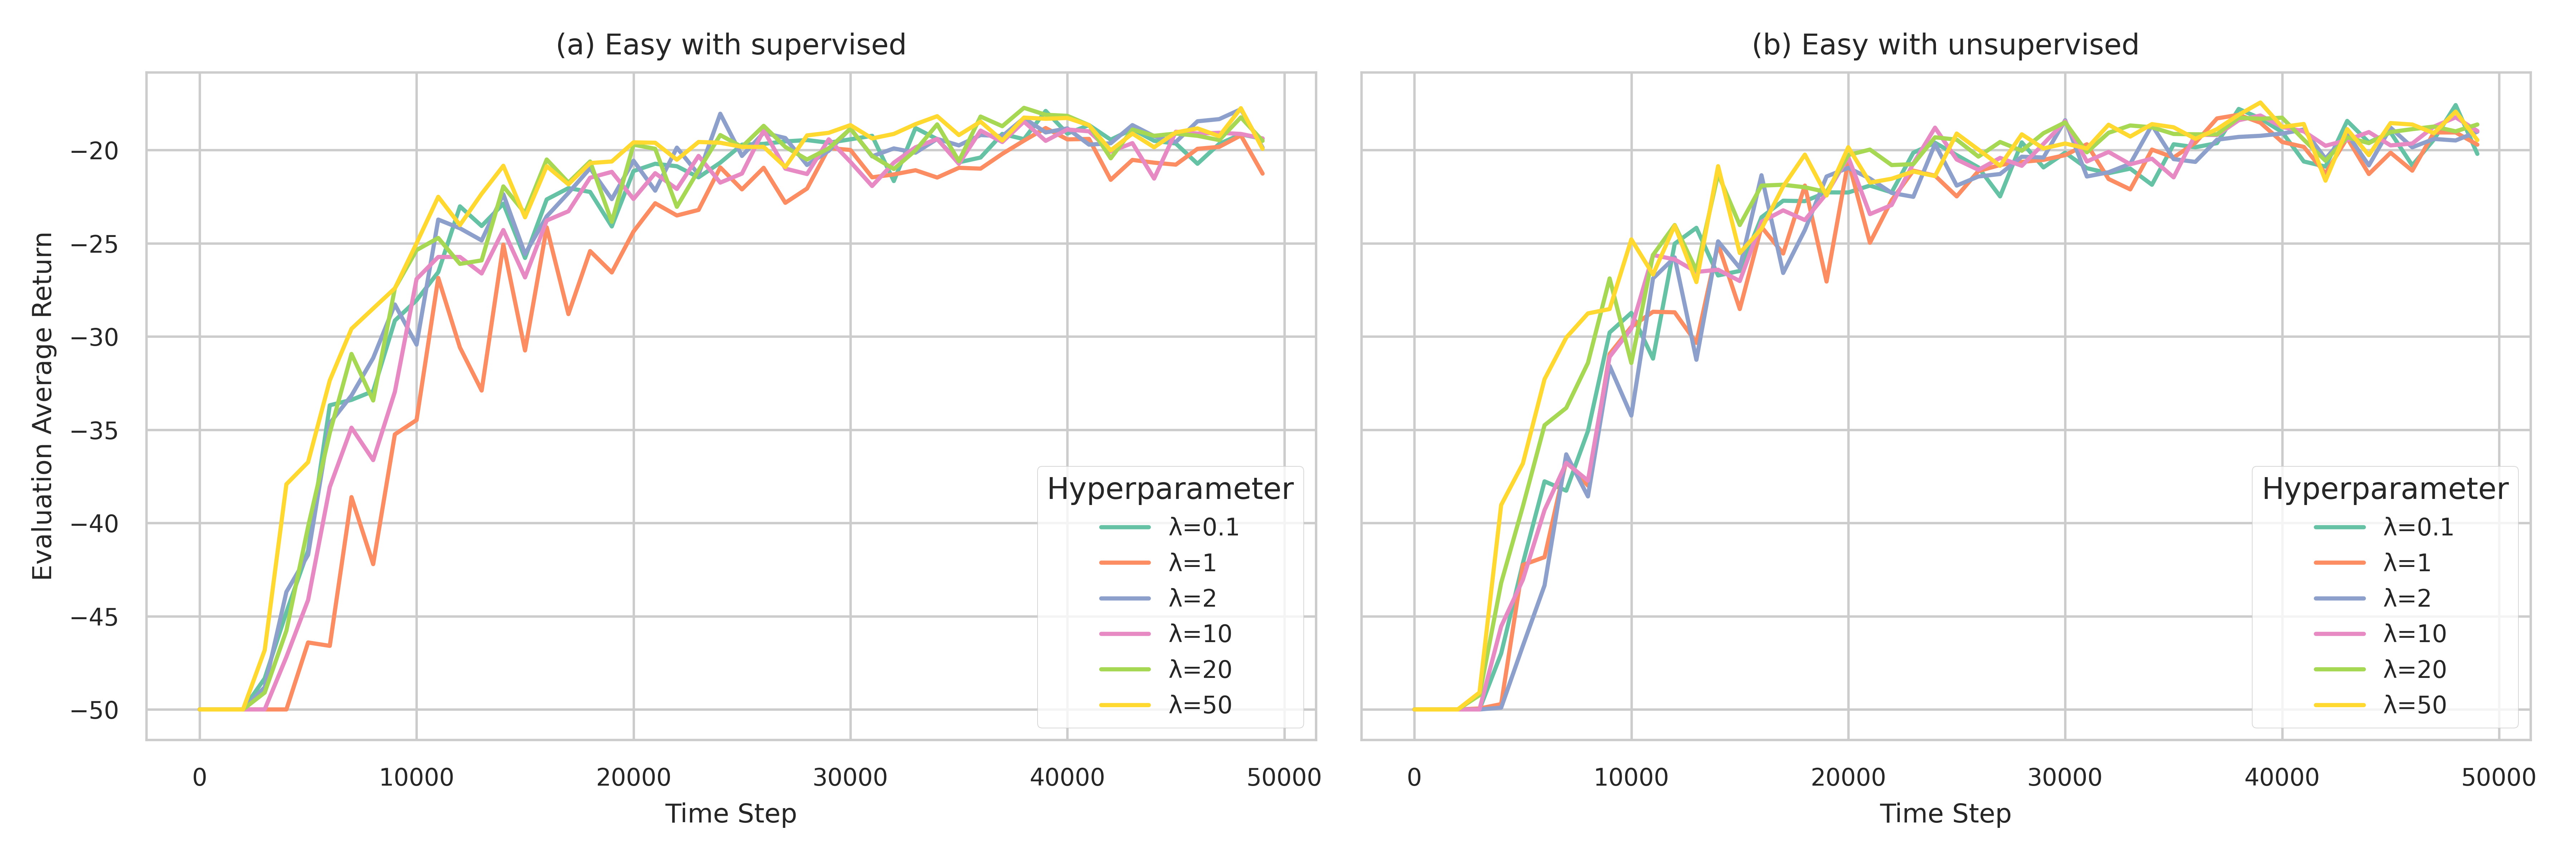
\includegraphics[width=\textwidth]{q4_easy.png}
    \caption{Learning curve from \texttt{PointmassEasy} environment: (a) supervised algorithm with different $\lambda$ settings; (b) unsupervised algorithm with different $\lambda$ settings. Explorations with supervised and unsupervised perform quite similar in this environment, which I think is partly due to the simplicity of the task. The best $\lambda$ settings for unsupervised and supervised explorations are both $\lambda=1$.}
\end{figure}

\begin{figure}[h!]
    \centering
    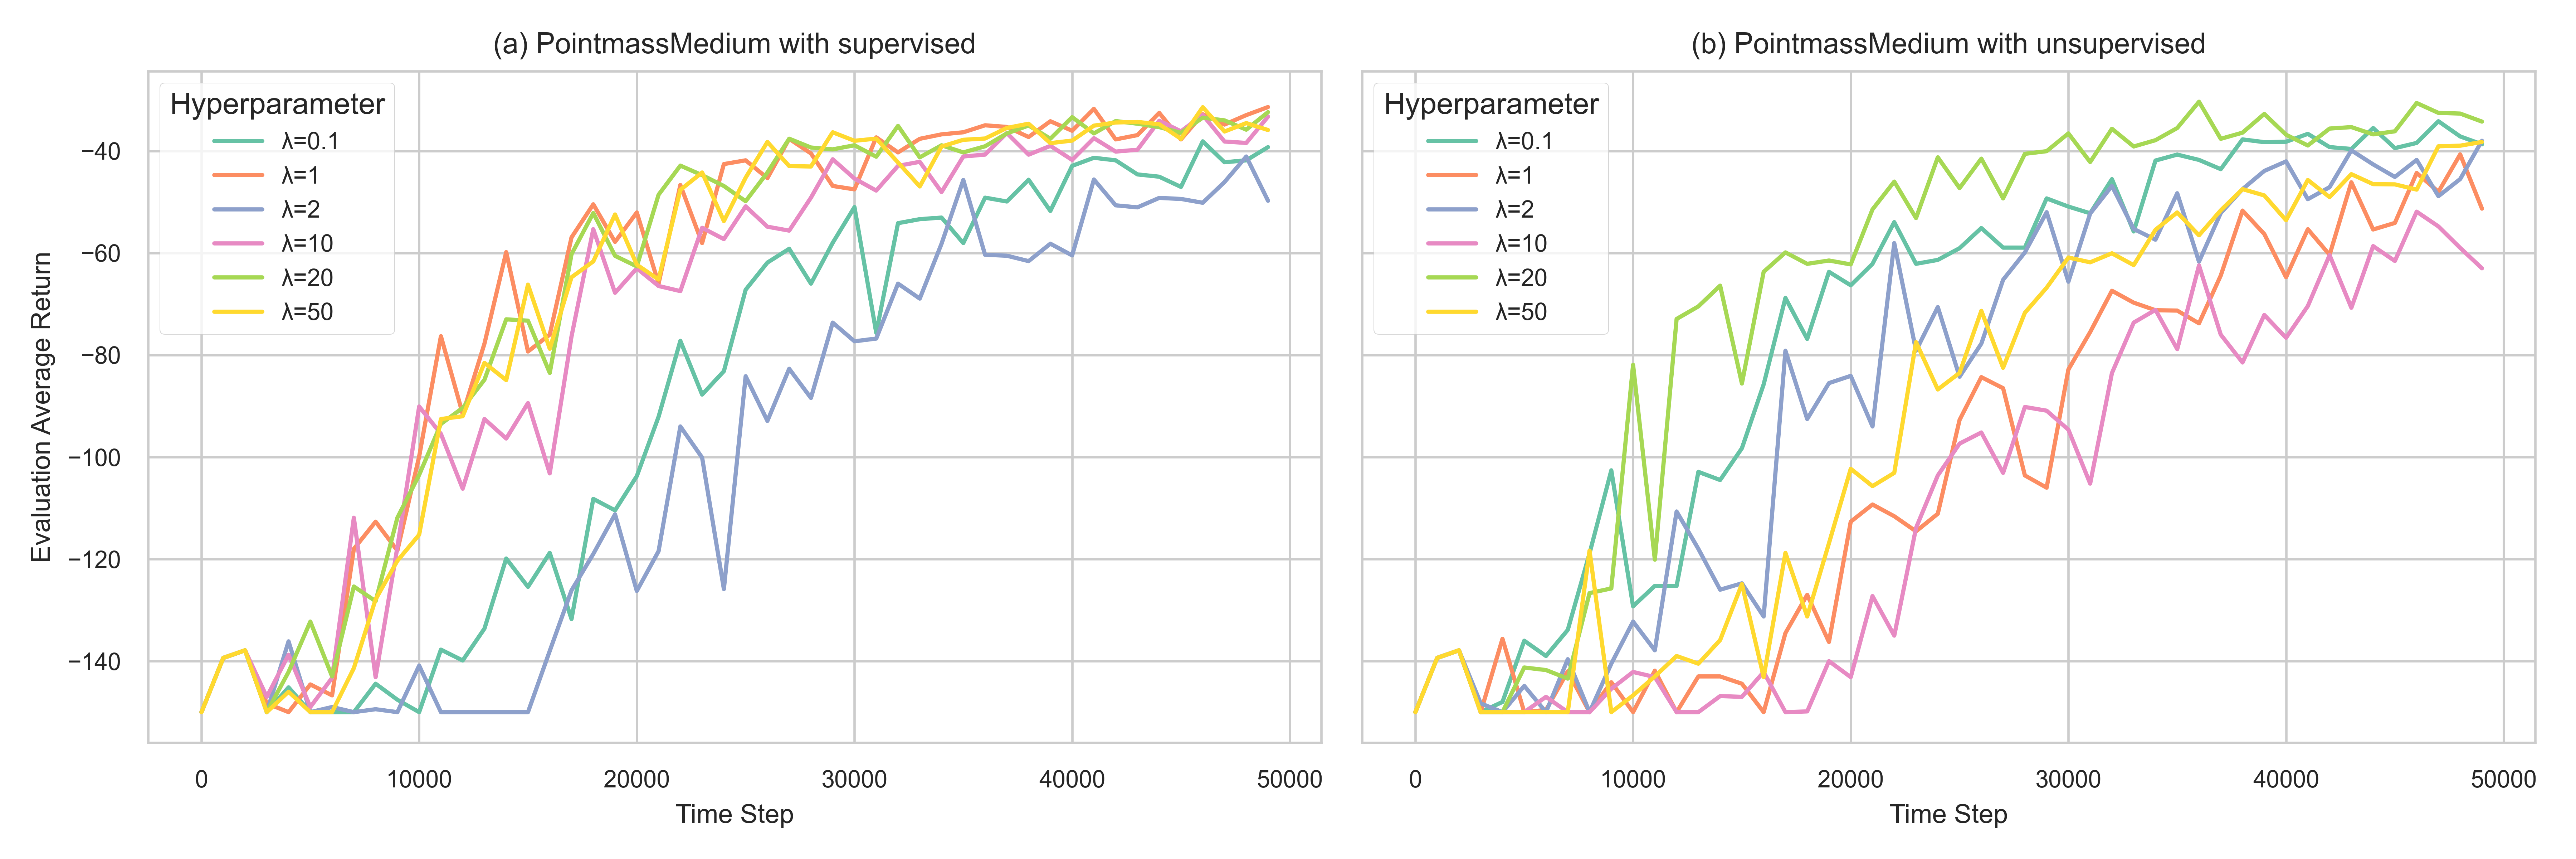
\includegraphics[width=\textwidth]{q4_medium.png}
    \caption{Learning curve from \texttt{PointmassMedium} environment: (a) supervised algorithm with different $\lambda$ settings; (b) unsupervised algorithm with different $\lambda$ settings. Training with supervised exploration is slightly better regarding the convergence speed. The best $\lambda$ setting for supervised and unsupervised RND are $\lambda=1$ and $\lambda=20$, respectively.}
\end{figure}

\pagebreak
\section*{Problem 5 Offline Learning with IQL}
\begin{figure}[h!]
    \centering
    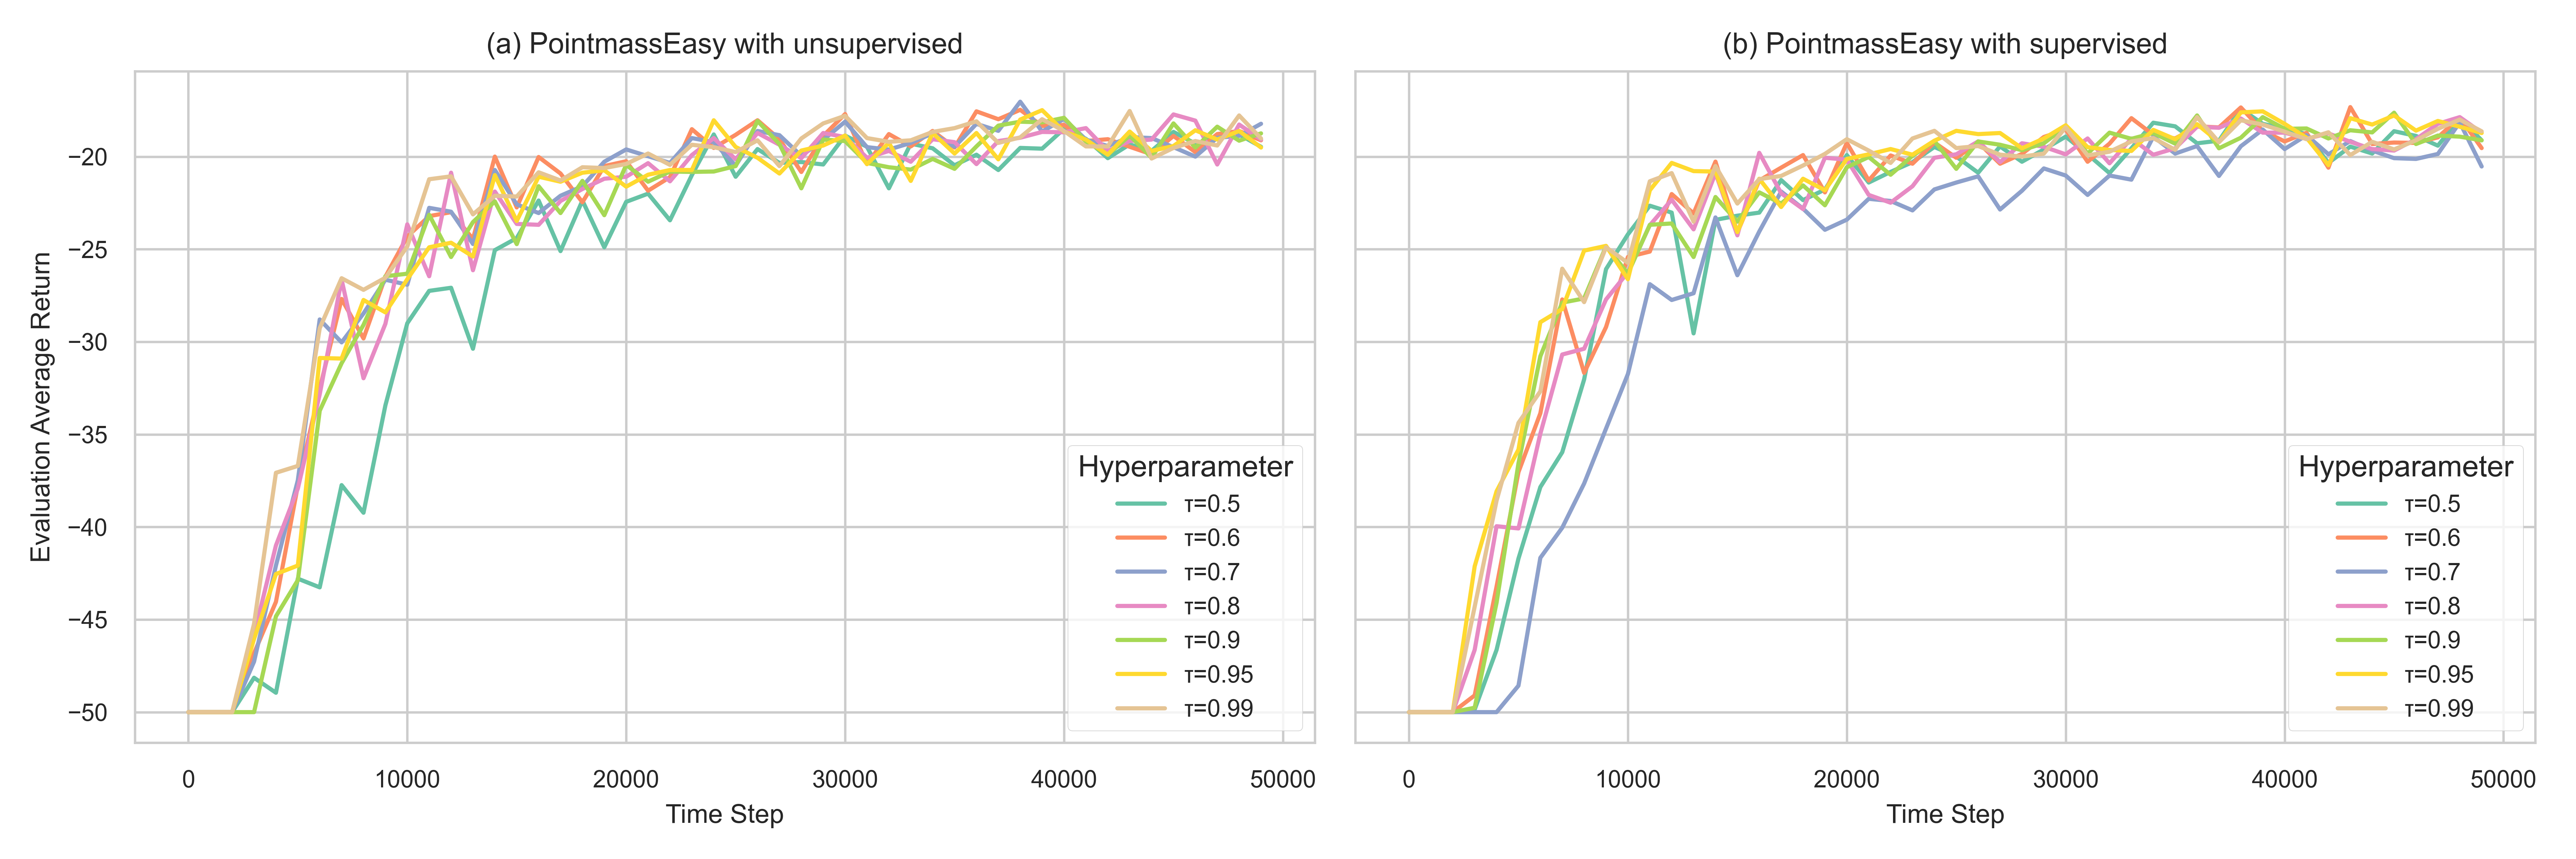
\includegraphics[width=\textwidth]{q5_easy.png}
    \caption{Learning curve from \texttt{PointmassEasy} environment: (a) supervised algorithm with different $\tau$ settings; (b) unsupervised algorithm with different $\tau$ settings. Increasing $\tau$ overall benefits the training but the marginal benefits decreases.}
\end{figure}

\begin{figure}[h!]
    \centering
    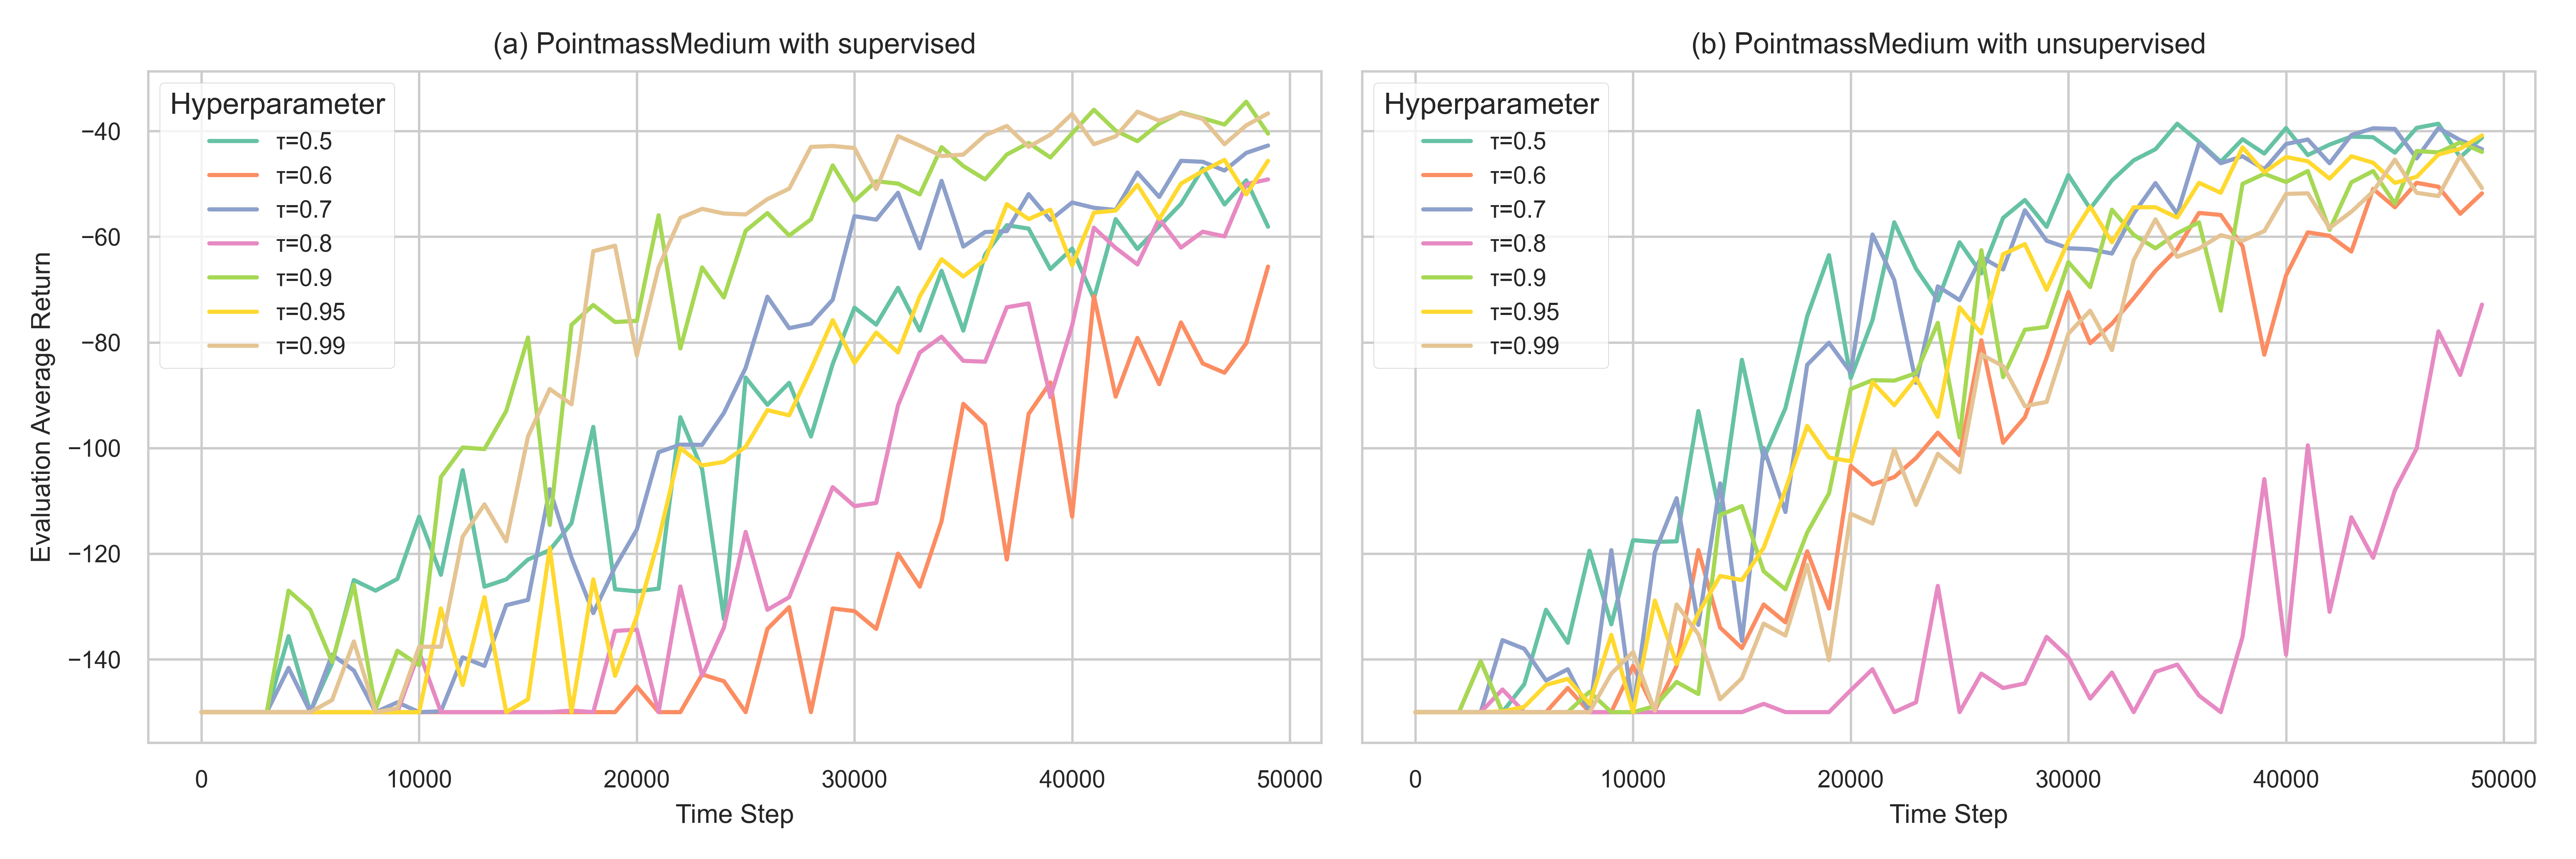
\includegraphics[width=\textwidth]{q5_medium.png}
    \caption{Learning curve from \texttt{PointmassMedium} environment: (a) supervised algorithm with different $\lambda$ settings; (b) unsupervised algorithm with different $\lambda$ settings. For supervised exploration, increasing $\tau$ overall benefits the training. But for the unsupervised exploration, increasing $\tau$ does not necessarily bring benefits. The optimal $\tau$ from my experiment is around $\tau=0.7$.}
\end{figure}

In summary, by comparing the learning curve from Problem 2 - 5, my experiment results show that IQL performs slightly better than the AWAC on the \texttt{PointmassMedium} environment, while almost the same on the \texttt{PointmassEasy} one. The two algorithm perform significantly better than the CQL algorithm.

\end{document}